\chapter{Prototypes d'application web pour la conception 3D collaborative}
\chaptertable

\section{Introduction}
Ce chapitre présente deux prototypes, chacun implanté sur un paradigme différent.
Le prototype 3DState repose sur des structure de données orientées états pour 
proposer une preuve de concept concernant principalement l'architecture de 
communication hybride, tandis que le prototype 3DEvent s'établi sur le paradigme 
événementiel pour implanter une approche peu couplée dans l'intergiciel \gls{P2P} 
et l'interface.orientée tâche par laquelle l'utilisateur interagit avec le système.
Chaque prototype possède les mêmes blocs : une interface utilisateur (contenant 
un environnement 3D) et un intergiciel \gls{P2P}.


La programmation réactive (PR) est le paradigme de programmation à la base de 
l'implantation des interfaces graphiques des deux prototypes : les composants 
répondent à des événements qui leur parviennent. 
Cela s'applique principalement à l'interface graphique mais 
également au niveau des flux réseaux pour proposer une application disponible 
(répondre rapidement), résilient (disponible même en cas d'erreur), souple 
(fonctionnel même surchargé), orienté messages (utiliser des messages 
asynchrones). Pour conserver ces propriétés, la programmation réactive impose 
de suivre la variation des valeurs dans le temps, être à l'écoute les événements 
qui surviennent, suivre les dépendances des variables pour pouvoir propager les 
mises à jour de valeurs, et enfin propager automatiquement les changements.
En cela, le langage de programmation \gls{JS} s'adapte bien à la PR car il repose 
sur un système de boucle d'événements, un gestionnaire d'événement et 
d'injection de comportements asynchrones. 

\paragraph{Signaling}
L'assomption est faite que tous les clients utilisent des navigateurs qui 
implémentent et supportent le protocole WebSocket et l'\gls{API} 
RTCDataChannel de WebRTC. Pour rappel, l'\gls{API} RTCDataChannel permet à 
chaque pair d'échanger des données arbitraires 
avec d'autres à partir du navigateur avec des propriétés de livraison 
personnalisables -- fiable ou non fiable (Section \ref{sec:fiabilite}), ordonné ou non 
ordonné (Section \ref{sec:ordre}). 
La connexion entre un pair (client) et le serveur est établie sur la base du protocole 
\gls{WebSocket}. Cette connexion bi-directionnelle est initialisée lors de la 
première requête du client pour récupérer le contenu de l'application. Cette 
connexion sert à la fois pour la phase de \textit{signaling} lors de l'établissement 
d'une connexion \gls{WebRTC} mais également pour que le client puisse envoyer 
des mises à jours originales à la base de données via les pairs reliés à la base de 
données. 


\paragraph{Interactions de base}
L'intérêt de proposer une application web se retrouve principalement dans 
l'accessibilité qu'elle propose. 
En effet, n'importe quel terminal muni d'un navigateur web peut y accéder, ce qui 
la rend distribuée et multiplateforme. 
Les fonctionnalités graphiques proposées par WebGL sont un peu réduites par 
rapport à celles d'OpenGL dont l'\gls{API} évolue plus vite et propose plus de 
flexibilité et d'optimisations. Cependant, les performances graphiques restent très 
correctes car le navigateur est quand même capable d'utiliser les processeurs 
graphiques du terminal (\gls{GPU}) pour les calculs et les rendus \gls{3D}.

Pour faire le lien entre le modèle et l'expérimentation, l'implantation du modèle a 
pris la forme d'un éditeur pour la modélisation \gls{3D} haut niveau permettant de 
visualiser et manipuler des objets \gls{3D} de manière collaborative dans un 
environnement web.

Dans chacun des prototypes, les interactions de bases sont les suivantes :
\begin{itemize}
	
	\item \textit{Visualiser, naviguer, utiliser les outils de transformation.} 
	L'utilisateur peut, 
	com\-me dans un environnement \gls{3D} classique, interagir avec la vue en 
	utilisant 
	la souris (survol, clic) et en bougeant la caméra (déplacements). Il peut 
	utiliser les commandes clavier et souris pour effectuer des opérations de 
	translation, de rotation et d'homothétie de trois manières différentes: 
	directement dans le \textit{viewport}, via le 
	menu ou via la console du navigateur.
	\item \textit{Charger des modèles \gls{3D}.} L'éditeur gère les formats de 
	fichier 3D les plus populaires (OBJ, PLY, DAE, glTF)
	\item \textit{Changement de référentiel.} La modification des coordonnées de 
	réfé\-ren\-ces (local/global)  pour les différentes transformations possibles
	\item \textit{Grid snapping} Cette fonctionnalité permet d'aligner les modèles 
	avec la 
	grille avec un effet de magnétisme sur les intersection de la grille.
	\item \textit{Changement de point de vue.} L'utilisateur peut à tout moment 
	passer de 
	son point de vue à celui d'un autre utilisateur. Le choix d'implanter ce type de 
	fonctionnalité s'inscrit dans la perspective de sensibilisation de l'utilisateur au 
	travail de ses collaborateurs. Ainsi, lors de la session, le fait de prendre le 
	point de vue d'un collaborateur est une manière de 
	comprendre son fonctionnement et d'imaginer ses 
	perspectives de conception à travers l'angle de caméra qu'il aura choisi.
\end{itemize}

Ces interactions, communes aux deux prototypes présentés, ne 
représentent cependant pas l'entièreté des fonctionnalités nécessaires à un 
environnement pour la manipulation d'objets 3D de manière 
collaborative. Par exemple, les fonctionnalités d'historique et de sensibilisation à 
la collaboration sont plus développées dans 3DEvent que dans 3DState.


Les travaux présentés s'inscrivent dans un contexte où les besoins 
d'interopérabilité et de standardisation sont élevés pour permettre à des 
utilisateurs de prendre le système rapidement en main sans installer autre chose 
qu'un navigateur.
\section{3DState : une preuve de concept orientée états}
\label{sec:3DState}
3DState correspond au prototype de 
\cite{Desprat2015a,Desprat2015b}. Il présente l'implantation de l'architecture de 
communication orientée états ainsi que les choix techniques qui l'accompagne.


%\subsection{Implantation des composants pour la communication}

\subsection{Implantation des composants pour la 
	communication}
		\paragraph{Serveur}
		
Le prototype utilise un serveur Node.js qui sert à la fois de serveur de 
\textit{signaling} pour mettre en liaison les utilisateurs mais il sert également 
de lien avec la base de données. Node.js permet d'utiliser du \gls{JS} côté 
serveur, simplifiant la compréhension et la maintenance de l'environnement. 
L'application utilise le micro-framework ExpressJS par dessus Node.js qui a 
l'avantage de simplifier le routage réseau.

		\paragraph{Base de données}

Pour assurer la sauvegarde au long-terme des modifications faite par les 
utilisateurs, la base de données MongoDB stocke l'état de chaque scène de 
l'application. L'utilisation d'une base de données NoSQL orientée document 
permet de stocker toutes les données pertinentes ensemble, dans un même 
document. Un document est auto-descriptif et peut imbriquer des données 
dans une structure d'arbre hiérarchisé. Une collection regroupe des 
documents. Dans ce prototype, il existe trois collections : \textit{Scenes} et 
\textit{Geometries} et \textit{Meshes}. 
La collection \textit{Scenes} contient chaque document concernant une 
scène : identifiant de la scène, métadonnées de l'espace virtuel (nom de la 
scène, liste des utilisateurs), liste des maillages inclus (identifiant maillage). 
La collection \textit{Geometries} comprend les géométries importées dans 
l'application sous la forme de : identifiant de la géométrie, données 3D.
La collection \textit{Meshes} représente les maillages utilisés dans les 
scènes : identifiant du maillage, nom du maillage, identifiant de la géométrie.
Les paramètres liés aux opérations \gls{CRUD} de la base de données sont 
fournis part la requête \gls{REST}. 

		\paragraph{Couche \gls{P2P}} 

La compatibilité entre navigateurs 
(cross-plateforme) concernant 
l'\gls{API} Datachannel issue du standard \gls{WebRTC} n'est pas encore 
effective. C'est pourquoi ce prototype ne fonctionne que sur les dernières 
version de Chrome (v49+), Firefox (v55+) et Opera (v47+). 
PeerJS\footnote{PeerJS  \url{http://peerjs.com}} est une 
bibliothèque \textit{open source} qui enveloppe WebRTC et fournie une \gls{API} 
de connexion navigateur-à-navigateur.
Le client possède un identifiant, donné par le serveur de \textit{signaling} lors 
de sa première connexion, qui lui permet de se connecter à un pair distant 
dont il a obtenu l'identifiant par le serveur. Le mécanisme 
de \textit{signaling} est délégué à PeerJS qui se charge de l'implantation de 
\gls{ICEF} et des problématiques \gls{NAT}. 


		\paragraph{Couche applicative}
		
Les différentes actions utilisateurs sont relayés par un système 
événementiel. L'interface intègre une couche de messagerie pour notifier les 
composant d'un nouvel événement \gls{JS}. Dans le prototype, la 
bibliothèque 
\textit{js-signals} sert de gestionnaire d'événements aux différents 
composants de l'\gls{IU} pour 
communiquer. Dans ce contexte chaque \textit{signal} possède un 
contrôleur, qui simplifie le contrôle de la réaction des événements en 
fournissant des fonctionnalités de souscription et de diffusion aux
événements~\gls{JS}. 

En comparaison avec une implémentation \textit{Event 
emitter / dispatcher} et \gls{PubSub}, le patron de conception 
Observateur dans \textit{js-signals} n'utilise pas de chaîne de caractère pour 
décrire les types d'événements \gls{JS} (évite les erreurs).
Une instance \textit{signal} enregistre des procédures (événements \gls{JS}, 
callbacks) qui peuvent être asynchrones. 
Lorsqu'il est intercepté -- n'importe où dans le contexte de l'application -- les 
procédures qui lui sont associées sont également déclenchées.

%\subsection{Interface de 3DState}
\subsection{Interface de 3DState}
L'implantation de l'interface a une forte dépendance avec les contraintes liés au 
rendu 3D dans le navigateur. Le framework ThreeJS a été choisi pour utiliser 
WebGL qui utilise le paradigme impératif, largement adopté dans la communauté 
du web 3D.

La Figure \ref{fig:3Dstateinterface} représente l'interface de l'éditeur implanté. 
l'utilisateur à accès a une liste des scènes. Lorsqu'une scène est sélectionnée elle 
est présentée ainsi : titre de la scène, nom des collaborateurs présents, outils 
d'édition, environnement 3D, détails de la scène et informations liées au client.


Dans ce prototype, présentant une preuve de concept pour l'architecture de 
communication orientée état, les outils d'édition sont représentés de manière 
rudimentaire. Les trois actions possibles sur un objet sélectionné sont 
représentées par les boutons \og translate\fg{} (translation), \og rotate\fg{} 
(rotation) et \og scale\fg{} (homothétie). Les actions peuvent être faites dans le 
repère \og local\fg{} ou dans le repère \og monde\fg{} selon l'état de la case à 
cocher \og local\fg{}. L'utilisateur à peu de retours indiquant le résultat de ses 
actions.

\begin{figure}
	\centering
	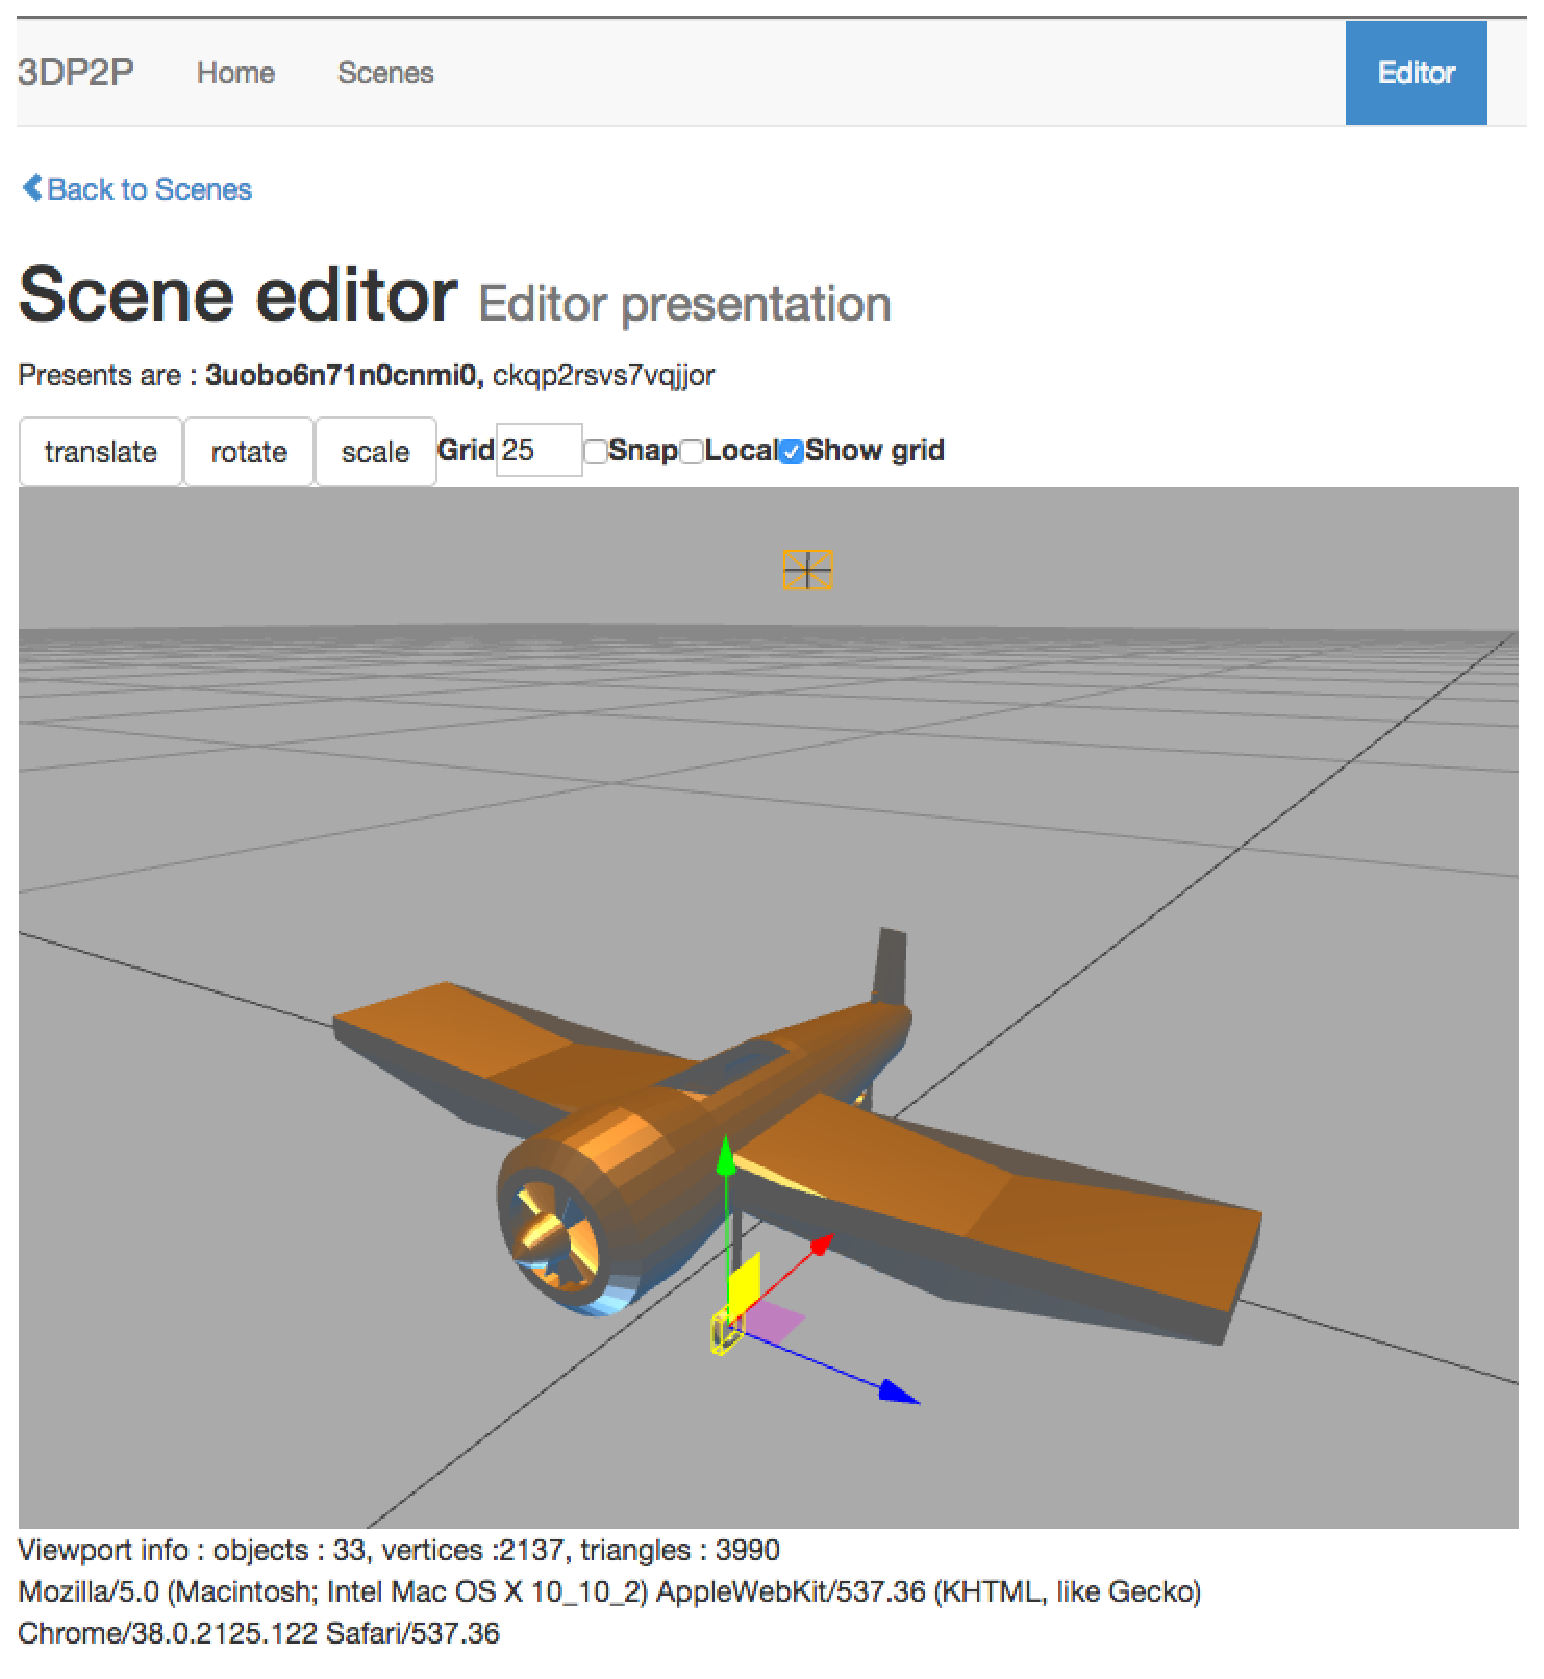
\includegraphics[width=0.6\columnwidth]{eps/editorpresentation.eps}
	\caption{Interface de 3DState}
	\label{fig:3Dstateinterface}
\end{figure}

\subsection{Gestion de la session}
\begin{figure}[h]
	\centering
	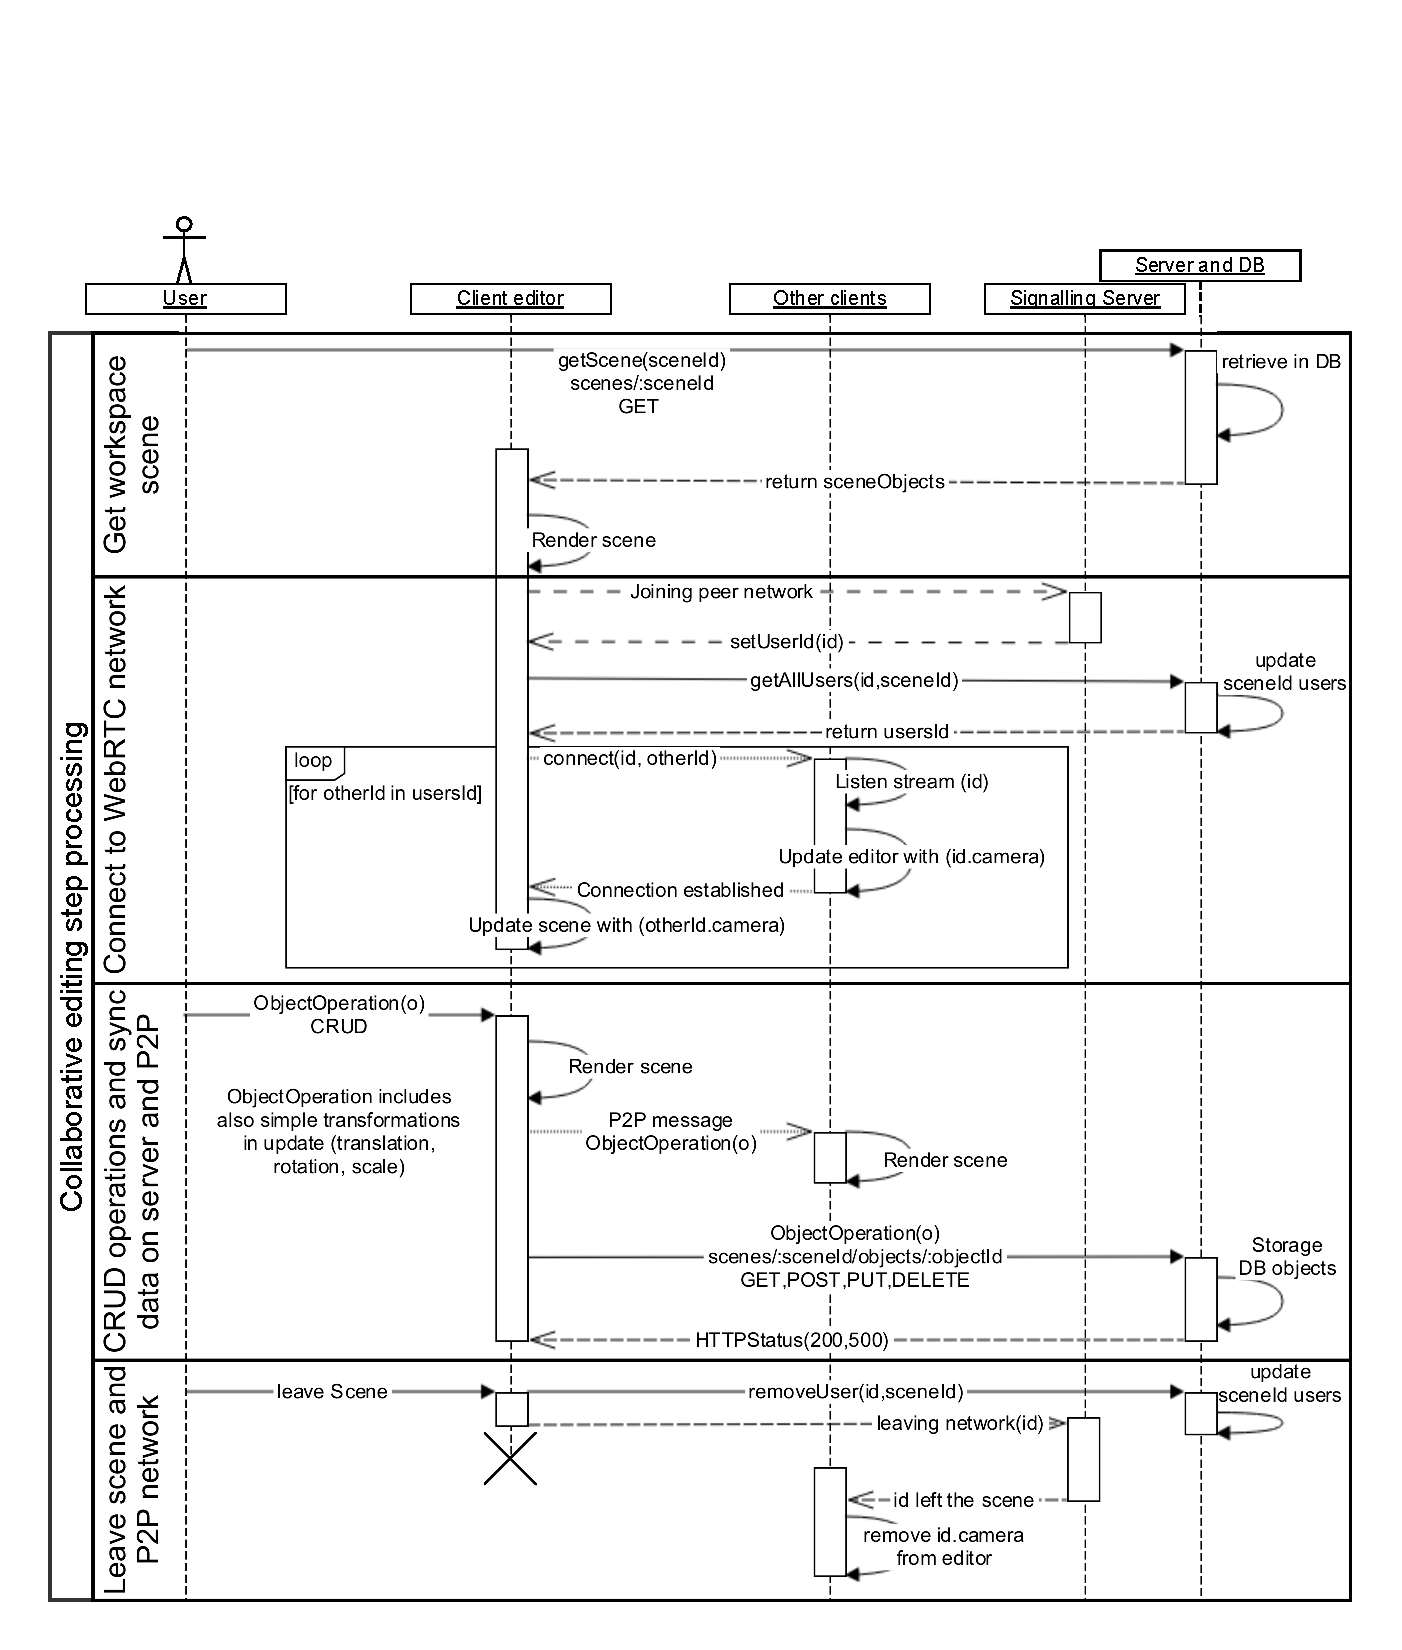
\includegraphics[trim={0 0 0 3cm},clip,width=0.9\columnwidth]
	{eps/sequence_wscg.eps}
	\caption{Diagramme de séquence de la gestion de la session dans une 
		architecture \og orientée état\fg{}}
	\label{fig:sequence_state}
\end{figure}
Lorsqu'un utilisateur rejoint une session, il suit le déroulement des opérations 
décrit dans la Figure \ref{fig:sequence_state}. 
Dans un premier temps, afin de récupérer les données liées à l'espace de travail, 
le client web de l'utilisateur qui se rend sur une scène récupère 
tous les objets associés à la scène dans la base de données. Les objets de la 
scène sont renvoyés à l'éditeur pour les afficher. 
Dans un second temps, le système établit les connexions \gls{P2P} entre les 
clients de manière automatique et complète (topologie réseau en maillage 
complet) après avoir récupéré les identifiants des autres utilisateurs auprès du 
serveur de \textit{signaling}. Une fois la connexion établie, chaque collaborateur 
voit son environnement \gls{3D} dans l'éditeur mis à jour, indiquant la position du 
nouvel 
arrivant. Les collaborateurs éditent ensuite la scène \gls{3D} qui produit, sur les 
différents objets, des requêtes \gls{CRUD} -- incluant les opérations de translation, 
rotation et homothétie -- destinées au serveur (qui transmet les 
modifications à la base de données) puis aux collaborateurs.
Enfin, dans un dernier temps, lorsque l'utilisateur quitte la scène, il en notifie le 
serveur de \textit{signaling} qui s'occupe d'indiquer aux clients restants l'abandon 
du client pour qu'ils puissent mettre à jour leur interface en conséquence.



		
		\subsection{Bilan critique}
Le prototype 3DState est issu de l'implantation de \cite{Desprat2015a} qui 
présente une architecture de communication hybride pour la modélisation 3D 
collaborative. Ses principales fonctionnalités sont : la mise en relation des clients, 
l'utilisation d'une interface web pour visualiser / ajouter / modifier des modèles 
dans une scène 3D. Chaque scène peut accueillir plusieurs collaborateurs et 
permettre à chacun de voir les modifications en temps réel des autres. La couche 
applicative utilise la programmation événementielle pour que les composants de 
l'application réagissent directement aux modifications des objets dans 
l'environnement 3D. 

L'implantation naïve que propose ce prototype pose plusieurs problèmes. 
D'une part, l'interface étant restreinte au minimum, il manque plusieurs 
fonctionnalités fondamentale pour que la modélisation collaborative s'effectue 
dans un environnement adéquat. Par exemple, il n'y a pas de liste 
des objets présents dans une scène et l'historique de la scène est également 
absent. La sensibilisation à la collaboration est quasiment absente (couleur 
différente par collaborateur) à l'exception de la représentation des collaborateurs 
par leur caméra dans l'environnement 3D. Stocker les éléments 3D par 
leur état impose un mise en mémoire coûteuse et des transferts d'autant plus 
coûteux par RTCDatachannel. Le Tableau \ref{table:3DStateChoixTechniques} 
résume les différents choix techniques effectués dans 3DState. 
		
			
			\begin{table}[!h]
				\centering
\caption{\label{table:3DStateChoixTechniques}Résumé des choix techniques pour 
3DState}
\begin{tabular}{llll}
	& \textbf{Plateforme / Service}& \textbf{Bibliothèque (version)}\\ \hline
	& \begin{tabular}[c]{@{}l@{}}
		Rendu WebGL \\ 
		Gestionnaire d'événements 
	\end{tabular} 	& 
	\begin{tabular}[c]{@{}l@{}}
		Three.JS (r69) \\ 
		signal-js (v1.0.0)
	\end{tabular}\\
	\multirow{-3}{*}{\textbf{Pair}} & WebRTC & PeerJS (v0.3.9)\\ \hline
	& Node.JS (v0.10.32)& ExpressJS (v4.9.0)\\
	& WebSocket & PeerJSServer (N/A) \\
	\multirow{-3}{*}{\textbf{Serveur}} & Base de données NoSQL & MongoDB 
	(v2.6.8) \\ \hline
\end{tabular}
\end{table}
			
			\paragraph{Testabilité}
La testabilité de l'application est nulle car tous les composants sont fortement liés 
entre eux. Cela ne permet pas de tester proprement les différents blocs du 
prototype. La collaboration est compliquée à observer dans un environnement 
implanté comme 3DState car l'approche orientée états ne rend pas compte des 
intentions des utilisateurs.

\section{3DEvent : une approche découplée orientée événements}
\label{sec:3DEvent}
Dans le chapitre précédent, une des contributions présentées correspond au 
modèle orienté événements : le \gls{framework} 3DEvent. 
L'implantation d'un tel système contient plusieurs éléments comme l'éditeur 
web et son interface utilisateur. Les éléments de sensibilisation à la collaboration 
sont également implantés comme le mécanisme de sélection multiple. Enfin, le 
système de visualisation flexible est un composant qui s'intègre du côté de la 
partie lecture en \gls{CQRS} pour proposer un contenu adapté au client. 


%\subsection{Intergiciel pour l'échange de 3D par événements}
\subsection{Intergiciel pour l'échange de 3D par événements}

L'architecture de communication décrite dans le chapitre précédent nécessite 
l'implémentation d'un intergiciel \gls{P2P} compatible avec les besoins liés à la 
3D, le web et la collaboration. Cette section décrit les politiques de connexion 
pour l'éditeur présenté dans la section précédente ainsi que les mécanismes de 
synchronisation nécessaire à l'échange de données dans l'application. 

\subsubsection{\textit{Signaling} et connectivité}
L'assomption est faite que tous les clients utilisent des navigateurs qui 
implémentent et supportent le protocole WebSocket et l'\gls{API} 
RTCDataChannel. 

La topologie de l'architecture de communication repose sur la mise en relation 
automatique des clients par le biais du serveur pour établir une connexion 
\gls{WebRTC}. Pour ce faire, chaque client envoie son identifiant (ID) lors de sa 
première requête au serveur qui le stocke. Selon le paramétrage de la connectivité 
directe minimum établie préalablement, le serveur recherche aléatoirement l'ID 
d'autres clients qui satisfont la règle de connectivité. Cette règle de connectivité 
minimum permet d'ajuster la densité du maillage (connectivité élevée: maillage 
partiel dense, voire complet ; connectivité faible: maillage partiel éparse) et 
d'obtenir une topologie maillée adaptée aux besoins de l'application en termes de 
synchronisation (temps-réel ou non) ou aux capacités des appareils. Il faut noter 
cependant que plus la connectivité est faible, plus l'information a besoin de 
transiter par des intermédiaires pour atteindre tous les pairs et par conséquent le 
temps de transmission est augmenté (exemple d'une distribution en ligne). 


Lors de la phase de \textit{signaling} c'est donc la partie gestion des instances du 
serveur qui gère la politique de connexion des données. Dans le prototype réalisé 
la connectivité minimum entre les différents pairs participant à la même scène est 
fixée à 2. Cette politique permet de créer un maillage réseau qui n'est pas trop 
dense en considérant que le nombre maximum d'utilisateur ne dépassera pas dix.

\subsubsection{De navigateur à navigateur}
Lors de la connexion d'un nouveau client à la scène, le serveur effectue la phase 
de \textit{signaling} permettant de le mettre en relation avec un autre client. Le 
mécanisme est répété tant que la règle de connectivité peut s'appliquer. Le client 
reçoit une notification de l'établissement de la connexion avec un autre client ce 
qui lui permet de démarrer l'échange de données.

Dans 3DEvent, le choix d'avoir un transport fiable et non ordonné a été fait pour 
respectivement garantir l'arrivée d'une donnée émise par l'utilisateur au sein de 
l'application et permettre des échanges asynchrones\todo{add \S sur "en cas de 
défaillance? }.
En cas d'arrêt soudain du serveur, si une connexion a été établie préalablement 
entre les clients et est toujours en cours, elle n'est pas impactée par la défaillance 
du serveur.
\subsubsection{Données d'échanges}

En sachant que le modèle est conçu pour des applications web, 3DEvent a besoin 
d'un format de données permettant de faire communiquer des acteurs hétérogènes 
du système.
Le format \gls{JSON} est assez générique pour être aussi utilisé lors de la 
sérialisation et la désérialisation des 
événements et plus largement des paquets transmis par RTCDataChannel. 
L'\acrshort{API} RTCDataChannel supporte beaucoup de types de données 
différents (chaînes de caractères, types binaires : Blob, ArrayBuffer\dots). Dans 
un environnement multi-utilisateurs tel que 3DEvent avec des données 
hétérogènes (3D, images, 
informations) l'interopérabilité est facilitée.

Le Listing  \ref{jsonstore} représente la structure de données utilisée sur le réseau 
lorsqu'un événement est transmis. Seule la partie $data$ est utilisée au sein du pair 
pour faire les manipulations en \gls{CQRS} car le type de l'instance d'événement 
manipulé est connu. 

La structure représentant l'événement transporte un numéro de version \og 
attendue\fg{} 
qui correspond à la version que l'agrégat doit avoir lorsque l'événement lui est 
appliqué. De cette manière la cohérence interne du pair est maintenu grâce à ce 
numéro de version.
Les événements contenant les objets 3D ($importGeometryEvent$) ont une 
propriété contenant la géométrie sous la forme d'un Blob contenant le fichier. 

\begin{lstlisting}[language=json,firstnumber=1,label=jsonstore,caption=Format
du Message transitant sur le réseau contenant l'événement MeshAddedToScene 
et ses 
paramètres]
{
	"packetId" : "567826g6-766b-f0g9676b677r",
	"streamId" : "scene-turbine",
	"eventType" : "MeshAddedToSceneEvent",
	"version" : 17,
	"data" : {
		"sceneId": "scene-turbine",
		"meshId":"406514c6-306b-f0f9643a037e",
		"geometryId": "37076875-ea1c-bbd300481345",
		"name": "blade",
		"color": "#963912",
		"author": "Foo"
	}
}
\end{lstlisting}


\subsubsection{Synchronisation des données}
\paragraph{Persistance à court terme}
Le navigateur (client) offre un espace de stockage avec l'interface \textit{Storage} 
de l'API Web Storage qui donne accès au \texttt{session storage} ou au  
\texttt{local storage}. Ce stockage est présent sur le client et fonctionne sur un 
système de clé / valeur. La configuration du client est également 
stockée localement. Grâce à ce système, il est possible d'avoir une 
persistance des données à travers les sessions du navigateur. Le contenu stocké 
correspond aux données générées par un utilisateur et par ses collaborateurs. Les 
répliques stockées sur chaque navigateur permettent à un utilisateur une plus 
grande 
autonomie en cas de déconnexion. C'est également un moyen de distribuer entre 
les clients les 
mises à jour qu'ils génèrent grâce au protocole de 
\gls{streaming3D} (cf. \ref{streamingprotocol}) sans passer par le serveur.

\paragraph{Protocole de streaming pour la synchronisation}
\label{streamingprotocol}

Il existe plusieurs méthodes de transmission de contenu au sein d'un réseau 
\gls{P2P} que l'on peut catégoriser selon deux modes : le téléchargement 
(\textit{download}) 
et le flux continu (\textit{streaming}). Le téléchargement requière que le contenu 
soit entièrement téléchargé pour pouvoir être lu, tandis que le flux continu peut 
être lu au fur et à mesure de sa récupération. Ce dernier mode, principalement 
utilisé pour la lecture de vidéo en ligne, s'applique bien à la transmission de 
contenu \gls{3D} : niveaux de détails \cite{Chu2012,Hu2008}, progressif 
\cite{Cheng2009,Limper2014}, mise en cache \cite{Jia2014}, compression / 
décompression
\cite{Lavoue2013,Ponchio2015,Maglo2013a}. 
Une catégorisation plus précise du flux continu peut être donnée selon la manière dont le 
contenu est généré : 
en direct (\textit{live} ou \textit{push}) et à la demande (\textit{on-demand} ou 
\textit{pull}).  
\todo{finir: 
	chaque client receptionne les info qui l’interesse : une scene en priorite?
	les messages sont stockes localement
	chaque client s’occupe de maintenir sa coherence
	et s’interroge les uns les autre pour coherenc e globale.
	->bcp de messages emis}



\subsubsection{Gestion des événements des agrégats}

Une connexion RTCDataChannel peut être configurée selon 
les critères (Section \todo{ref section config}) de fiabilité et d'ordonnancement. 
Dans l'intergiciel de 3DEvent, cette configuration est : non fiable et non ordonnée. 
C'est l'application qui est en charge de \og ré-ordonner\fg{} les événements. En 
effet, les événements sont associés à des agrégats. Comme chaque agrégat 
possède un flux d'événements dédié et numéroté il est alors simple pour 
l'application de les 
ordonner lorsqu'elle les réceptionne. 
Lors de la synchronisation (Section \todo{ref section sync}), les 
événements manquants sont demandés successivement à tous les pairs. Lors 
qu'un pair reçoit les événements il les stocke dans le flux correspondant à 
l'agrégat. Si un événement est manquant, les suivants sont quand même stockés 
en laissant l'espace de l'événement manquant dans le tableau. L'événement est 
redemandé jusqu'à son obtention, laquelle provoque le déblocage de l'état de 
l'agrégat jusqu'au prochain événement manquant (ou la fin du flux). Les 
événements qui ont été stockés \og en attendant\fg{} permettent à l'application 
d'être directement en capacité de poursuivre la construction de l'état de l'agrégat. 
Cette mécanique tire avantage des Snapshots (présentés dans \todo{ref section}) 
qui réduisent la taille des flux en mémoire pour chaque agrégat qui part déjà d'un 
état avancé.\todo{mettre en avant cette partie}


\begin{figure}
	\centering
	\inputTikZ{0.9}{eps/tikz/streams/aggregate.tex}
	\caption{Exemple d'agrégats}{Structure d'un agrégat et ses versions. Chaque 
		version est un état de l'agrégat qui correspond à l'empilement des instances 
		d'événements (ei) qu'il contient. Les types des événements sont relatifs au 
		type 
		d'agrégat dans lequel il est contenu.}
	\label{fig:aggregate}
\end{figure}
%\subsection{Interface orientée tâche}
\subsection{Interface orientée tâche}
\label{sec:task-based-ui}
Dans le but de proposer une \gls{IU} proche des fonctionnalités métiers liées à la 
modélisation \gls{3D}, l'éditeur possède une interface orientée \og tâche\fg{}, en 
comparaison avec des \gls{IU} \gls{CRUD}. En effet, les \gls{IU} \gls{CRUD} 
réduisent la sémantique métier du domaine d'application à la création, la lecture, la 
mise à jour et la suppression, omettant toutes les subtilités que peuvent dégager 
ces actions en perdant l'intention de l'utilisateur dès le niveau de l'interface. Une 
interface orientée tâche a tendance à s'attarder sur toutes les nuances que le 
domaine possède en caractérisant chaque action sans subir d'effet de 
simplification. Cette proximité avec le métier permet de calquer directement 
l'interface du modèle événementiel sur l'\gls{IU} et de guider l'utilisateur dans ses 
activités. L'utilisabilité, qualité de l'expérience utilisateur fournit par un système 
pour réaliser une tâche, est alors maximisée en terme d'efficacité, d'efficience et 
de satisfaction. 
Ce type d'\gls{IHM} s'organise autour de cas d'utilisation. Cela permet, 
d'une part, de présenter clairement les 
actions (\og ajouter une géométrie à la 
bibliothèque à partir d'un fichier\fg{} plutôt que \og téléverser un fichier\fg{}) : 
l'intention est clairement définie. D'autre part, lorsque l'utilisateur s'apprête à faire 
une action, seules les informations utiles sont affichées. Enfin, l'application fournit 
simplement l'information dans le contexte où elle doit être présentée, évitant à 
l'utilisateur d'aller la chercher ailleurs.
L'\gls{IU} devient alors une couche de l'application qui nécessite d'agréger, croiser 
et filtrer des données. La dénormalisation proposée par \gls{CQRS} remédie à ce 
besoin dans le cadre de la consultation de données. 


\subsubsection{Présentation de l'interface}


%\begin{figure}[h!]
%	\centering
%	\begingroup
%	
%	\subfloat[Rotation (vue \gls{3D}) et outils de manipulation d'objet 
%	\gls{3D} 
%	(panneau 
%	
%latéral)]{\includegraphics[width=0.75\textwidth]{eps/2rotatedetail.eps}\label{fig:ui2}}\hfill
%	
%	\subfloat[Translation (vue \gls{3D}) et visualisation de l'historique 
%	(panneau 
%	
%latéral)]{\includegraphics[width=0.75\textwidth]{eps/1translatehisto.eps}\label{fig:ui1}}\hfill
%	
%	\subfloat[Mise à l'échelle (vue \gls{3D}) et liste des collaborateurs 
%	(panneau 
%	
%latéral)]{\includegraphics[width=0.75\textwidth]{eps/3scalecollab.eps}\label{fig:ui3}}\hfill
%	
%	\endgroup
%	\caption{Interface utilisateur pendant une session collaborative (trois 
%personnes)}
%	\label{fig:screenshots}
%\end{figure}
Lorsqu'un utilisateur se connecte à une scène, il a accès à une interface web 
(dans un navigateur) qui représente l'espace de travail collaboratif et qui lui 
permettant 
d'utiliser différentes fonctionnalités. Les deux modalités d'interaction sont le clavier 
et la souris\info{est ce qu'on parle de mobile?}. Le premier niveau de cette 
interface est scindée en deux panneaux~: 
\begin{enumerate}
	\item L'espace \gls{3D} consacré à la visualisation des objets et à leur 
	manipulation 
	dans l'environnement \gls{3D}~;
	\item La barre d'outils qui contient trois onglets~:~
	\begin{enumerate}
		\item "Scene" contient tous les détails de la scène et des maillages qu'elle 
		inclue~; 
		\item "Collaboration" fournit les informations liées à la collaboration~;
		\item "History" liste tous les événements qui ont eut lieu dans la scène et 
		leurs  détails. 
	\end{enumerate}
\end{enumerate}

\begin{figure}[]
	\centering
	\begingroup
	
	\subfloat[Onglet \og outils de manipulation sur la 
	scène\fg{}]{\includegraphics[width=0.38\textwidth]{eps/scenecontrol.eps}\label{fig:uicontrol}}
	\hfill
	\subfloat[Onglet \og collaboration\fg{}]
	{\includegraphics[width=0.27\textwidth]{eps/collaboration.eps}\label{fig:uicollab}} 
	\hfill
	\subfloat[Onglet \og 
	historique\fg{}]{\includegraphics[width=0.32\textwidth]{eps/history.eps}\label{fig:uihisotry}}
	
	\endgroup
	\caption{Onglets du panneau latéral de l'interface}
	\label{fig:uipanneau}
\end{figure}

La Figure \ref{fig:uipanneau} montre quelques captures d'écran durant une 
session collaborative sur le modèle Rotor. L'onglet "Scene" (Figure 
\ref{fig:uicontrol}) possède un bloc contenant les détails 
d'un 
maillage en cours de 
sélection. Cela permet d'avoir la description des propriétés de l'objet sélectionné et 
une manipulation de ses paramètres (position, rotation et mise à l'échelle) plus 
précise que via l'espace \gls{3D} avec le cliqué / déplacé. "Scene" intègre 
également un espace réservé aux géométries disponibles dans la scène appelé 
Bibliothèque (de géométries).

L'onglet "Collaboration" (Figure \ref{fig:uicollab}) présente la liste des 
collaborateurs qui 
participent à la 
scène. Chacun d'eux est décrit par son nom, son état  (connecté ou déconnecté) 
et son rôle (administrateur, éditeur, lecteur ou autre\footnote{Un rôle peut être 
	défini par le biais du \gls{framework} 3DEvent}). En cliquant sur un élément de 
	la 
liste, l'utilisateur accède au dernier point de vue dans l'espace \gls{3D} connu du 
collaborateur représenté.

L'onglet "History" (Figure \ref{fig:uihisotry}) liste tous les événements passés dans 
la 
scène en fournissant 
l'accès à leur détail. Pour chaque événement, le système est capable de montrer 
dans l'espace \gls{3D} la différence entre l'état  après l'événement cliqué $state_x$ 
et l'état courant $state_n$. L'utilisateur peut à partir de cette visualisation choisir 
de \og revenir en arrière\fg{} sans perdre les données entre $state_n$ et $state_x$ 
car dans le système présenté ici, cela s'effectue par compensation (cf 
Event-Sourcing 
Section X)\improve{annulation d'un événement ou juste ES}.

Dans chaque onglet se trouvent différents blocs \gls{HTML}, avec des 
comportements spécifiques à un agrégat et injectés dynamiquement. Ces blocs 
correspondent aux vues de ce modèle.

Parmi les vues disponibles dans le système, une grande partie est dédiée à 
l'\gls{IU} de l'application web pour le cas d'utilisation de la modélisation 3D. 
D'autres views sont disponibles pour un autre type d'utilisation destinée à 
l'observation des comportements des utilisateurs, élément primordiale dans 
une expérimentation.



\subsubsection{Exemple d'interaction}
La Figure \ref{fig:cqrs-example} décrit la façon dont le système traite l'exécution 
d'une commande de translation déclenchée par l'utilisateur et comment cette 
information est diffusée aux collaborateurs\footnote{Pour que l'exemple 
	fonctionne, la scène, la géométrie du cube et le maillage \textit{cube1} doivent 
	avoir été créés en amont.}.
Dans l'étape (a), la commande déclenchée par l'utilisateur s'adresse à l'agrégat 
$cube1$ et contient les paramètres de la translation (vecteur x, y, z). L'agrégat, 
qui 
modélise le domaine d'un maillage, génère l'événement de translation $e1$ (étape 
(b)) si tout est valide d'un point de vue métier. L'événement $e1$ est ensuite 
passé à l'Event Store. 
Le composant responsable de la détection de conflit permet au développeur 
d'implémenter ses propres règles de résolution de conflit. Le composant déclenche 
une exception lorsque le numéro de version reçu et le numéro de version courant 
de l'agrégat sont identiques (Figure \ref{fig:cqrs-example} étape (c)). Selon les 
règles métiers définies et les exceptions liées à la cohérence, l'événement peut 
être 
rejeté. Ce traitement peut être à l'origine de la génération de nouveaux 
événements.


\begin{figure}[]
	\centering
	\includegraphics[width=\columnwidth]{eps/example10.eps}
	\caption[Flux de la collaboration dans le framework 3DEvent entre 3 
	utilisateurs]{Exemple d'édition collaborative où User A est connecté à User  B, 
		lui 
		même connecté à User C. Le cycle montre les différentes étapes du 
		déclenchement: la commande, la 
		génération 
		de l'événement, la 
		synchronisation du journal d'événements, l'impact sur le rendu des autres 
		utilisateurs pour une translation sur un cube et le rendu 
		visuel.}\label{fig:cqrs-example}
\end{figure}

\subsection{Sélection fantôme}
Les interactions utilisateurs doivent être adaptées à la collaboration et aux 
manipulations à effectuer. Pour cela, l'éditeur 3DEvent introduit la fonctionnalité de 
sélection \og fantôme\fg{}. Lorsqu'un utilisateur souhaite sélectionner un objet de 
la scène, l'objet original ($O_o$) est 
cloné et devient l'objet fantôme ($O_f$). $O_f$ conservent les mêmes propriétés, 
représenté avec de la 
transparence d'où le terme \og fantôme\fg{}. 
L'objet $O_f$ prend alors le focus de sélection pour que l'utilisateur le manipule à 
la place de l'objet $O_f$. 
Lorsque l'utilisateur relâche $O_f$, alors la modification intentée s'applique sur 
$O_o$ avec le principe du \textit{Last Write Wins} (le dernier gagne).
La Figure \ref{fig:ghostselection} 
représente la sélection fantôme lors de la translation du corps du rotor par 
l'utilisateur Foo : c'est l'objet transparent qui est manipulé alors que l'objet opaque 
représente sa position originale. 
En différenciant l'actuel objet que l'utilisateur souhaite sélectionné ($O_{o}$) de 
celui manipulé ($O_f$), l'interaction est mise en valeur sous quatre angles :
\begin{itemize}
	\item l'ergonomie dans l'environnement \gls{3D} :
	$O_f$ est un objet temporaire qui permet à l'utilisateur
	d'avoir une visualisation de l'objet en cours de manipulation tout en 
	conservant le dernier état de $O_o$ visible. 
	$O_o$ peut être considéré comme un point de repère visuel pour l'utilisateur 
	lorsqu'il effectue sa manipulation. 
	L'$O_f$ a aussi un rôle d'intermédiaire entre l'utilisateur et la 
	finalité de l'interaction en donnant un support visuel à sa réflexion experte.
	Grâce à $O_f$, l'utilisateur peut également révoquer sa manipulation en 
	cours sans avoir eu d'impact sur $O_o$ en évitant des actions inutiles (faire 
	l'action 
	puis la défaire) pour le métier et coûteuses pour le réseau.
	
	\item la collaboration : si un collaborateur effectue une modification 
	à destination du même $O_o$ alors la représentation de $O_o$ chez 
	l'utilisateur est également modifiée. $O_f$ par contre ne subit pas d'impact ; 
	l'utilisateur peut continuer sa manipulation et~/~ou l'ajuster en fonction des 
	nouvelles informations liées à $O_o$ ou même révoquer sa manipulation 
	en cours si cela lui convient.
	
	\item le métier : seules les manipulations menées à terme sont 
	considérées comme des commandes. Cela évite d'avoir des événements qui ne 
	sont pas pertinents pour le métier dans le journal d'événements (comme lorsque 
	l'utilisateur change d'idée lors de l'interaction ou
	suite à une intervention concurrente). L'utilisateur n'a un impact sur l'application 
	que lorsqu'une modification métier est réalisée.
	
	\item le réseau : l'information importante à faire transité est l'événement 
	correspondant à la modification métier pas toutes les positions intermédiaires 
	même si intuitivement l'idée de temps réel pourrait conduire à cette solution. La 
	quantité de messages produite surchargerai à la fois le réseau et le fil 
	d'exécution principale de l'application. En effet, \gls{WebRTC} a l'inconvénient 
	pour le 
	moment de ne pas pouvoir s'exécuter dans un \textit{Web Worker} (fil 
	d'exécution 
	parallèle en JavaScript). Cette solution imposerai des 
	latences réseau et d'\gls{IU} qui affecteraient gravement l'expérience utilisateur
	sans apporter d'informations supplémentaires à l'aspect métier de la 
	collaboration. 
\end{itemize}


\begin{figure}[ht]
	\centering
	\includegraphics[trim={0 0 0cm 0}, clip, 
	width=0.8\columnwidth]{eps/1translatehisto.eps}
	\caption{Illustration de la sélection fantôme dans l'environnement 3D}{
		Les boîtes englobantes représentent la sélection des différents 
		collaborateurs pendant la session.
	}
	\label{fig:ghostselection}
\end{figure}

\paragraph{Projections}
\todo{refomuler}
chaque partie de l’interface est liée à une proj de la bdd
les actions user et les actions des autres users passent par le meme cycle
pas de diff de prise en compte des evnts de l’interaction user ou de la couche 
reseau
en CS : les actions users -> actions -> recup info
action push du servuer qui peuvent etre gerees de maniere diff
\subsection{Bilan}

\todo{refomuler}
L'application 3DEvent repose sur les principes et les 
technologies du web pour permettre de visualiser et manipuler des objets \gls{3D} 
de 
manière 
collaborative en temps-réel.
\paragraph{Testabilité}
\section{Conclusion du chapitre}


\section{Conclusion du chapitre}

Ce chapitre décrit l'implantation des contributions présentées dans le chapitre 
précédent.
Le premier prototype, 3DState est issu des premiers travaux de cette thèse. Son 
implantation repose principalement sur la mise en place des technologies 
nécessaires pour proposer une collaboration basique. L'interface proposé permet 
simplement de manipuler des objets 3D dans la scène sans intégrer par d'autres 
moyen les collaborateurs à l'exception du changement de point de vue. La gestion 
de la session se concentre principalement sur la mise en relation des utilisateurs 
et la récupération du contenu. Le client est donc très sollicité à chaque 
modification. L'utilisateur est assuré que ses messages envoyés sont reçu et 
grâce au mécanisme de verrouillage des objets sélectionné, les conflits sont nuls. 
Le transfert par différentiel d'état relève d'un calcul assez faible pour le client.

Le second prototype, 3DEvent, intègre un intergiciel \gls{P2P} permettant de faire 
communiquer différent types de plateformes entre elle grâce à l'implantation de 
webrtc-eventstore. Les différences entre les Instances Serveur, qui utilisent  
node-webrtc sur NodeJS, et les Instances Web, qui utilisent PeerJS sur le 
navigateur, sont alors abstraites par cette bibliothèque qui fait l'interface et leur 
permet de communiquer en \gls{P2P}. Cette solution technique ouvre de nouvelles 
perspectives quand à l'extension du \gls{P2P} dans les navigateurs, les mobiles, 
et les systèmes embarqués. Les propositions liées à l'interface orientée tâches 
sont en accord avec le modèle événementiel et permettent de focaliser les 
interactions des utilisateurs directement sur les tâches métier, c'est à dire les 
tâches de manipulation et de visualisation 3D collaborative. La synchronisation et 
la gestion de la cohérence dans un environnement décentralisé comme 3DEvent 
sont mis en place accompagnés de modules de sensibilisation à la collaboration 
comme la sélection fantôme.

Les deux prototypes ont été réalisés dans le but 
\begin{enumerate*}[label=(\roman*)]
	\item de montrer la faisabilité des 
	propositions liées aux contributions et
	\item de proposer des expérimentations 
	utilisateurs pour évaluer et valider les choix de conception et d'implantation des 
	modèles utilisés.
\end{enumerate*}
%
%4.3.1 Intergicielpourl’échangede3Dparévénements . . . . . . . . . . . . 91
%4.3.2 Interfaceorientéetâche.......................... 94
%4.3.3 Sélectionfantôme............................. 96
%4.3.4 Bilan